\chapter{Autoskalowanie}
\label{cha:autoscaling}

\section{Horizontal Pod Autoscaling}

\begin{figure}[!ht]
	\begin{center}
		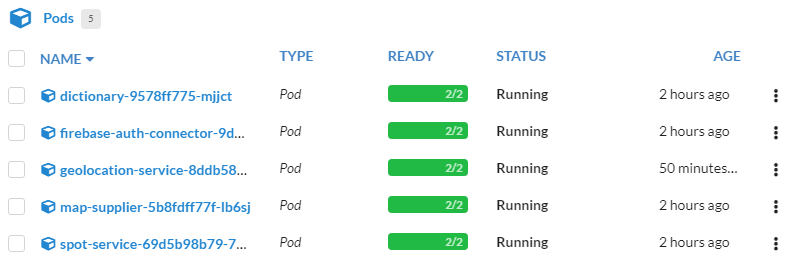
\includegraphics[width=0.9\textwidth]{img/autoscaling/hpa-pods-normal}
	\end{center}
    \caption{Spoczynkowy stan Pod'ów}
\end{figure}

\begin{figure}[!ht]
	\begin{center}
		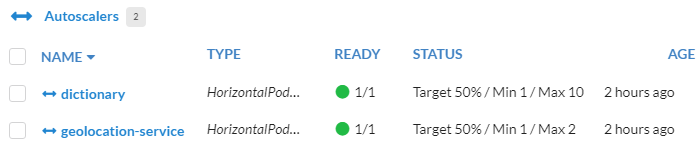
\includegraphics[width=0.9\textwidth]{img/autoscaling/hpa-autoscalers-normal}
	\end{center}
    \caption{Spoczynkowy stan Autoscaler'ów}
\end{figure}

\begin{figure}[!ht]
	\begin{center}
		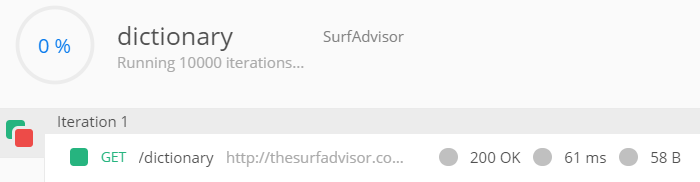
\includegraphics[width=0.8\textwidth]{img/autoscaling/hpa-dictionary-test-postman}
	\end{center}
    \caption{Test obciążeniowy \emph{dictionary-service} z Postmana}
\end{figure}

\begin{figure}[!ht]
	\begin{center}
		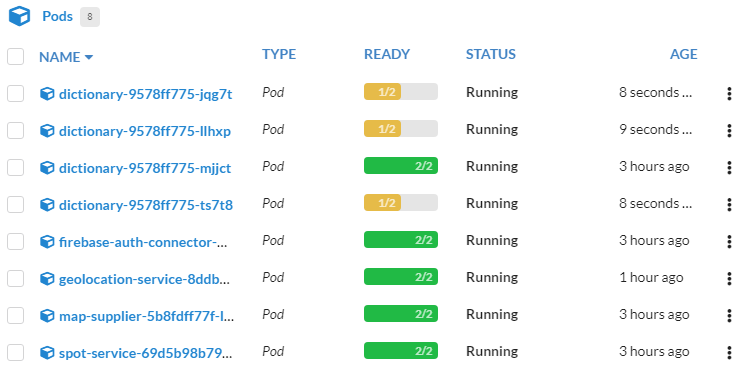
\includegraphics[width=0.9\textwidth]{img/autoscaling/hpa-pods-scale-up}
	\end{center}
    \caption{Stan Pod'ów przy skalowaniu w górę}
\end{figure}

\begin{figure}[!ht]
	\begin{center}
		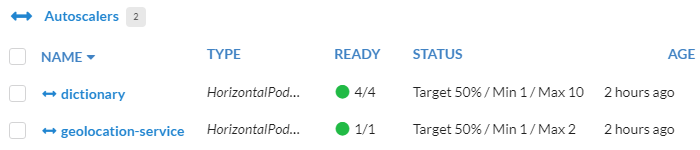
\includegraphics[width=0.9\textwidth]{img/autoscaling/hpa-autoscalers-scale-up}
	\end{center}
    \caption{Stan Autoscaler'ów przy skalowaniu w górę}
\end{figure}

\begin{figure}[!ht]
	\begin{center}
		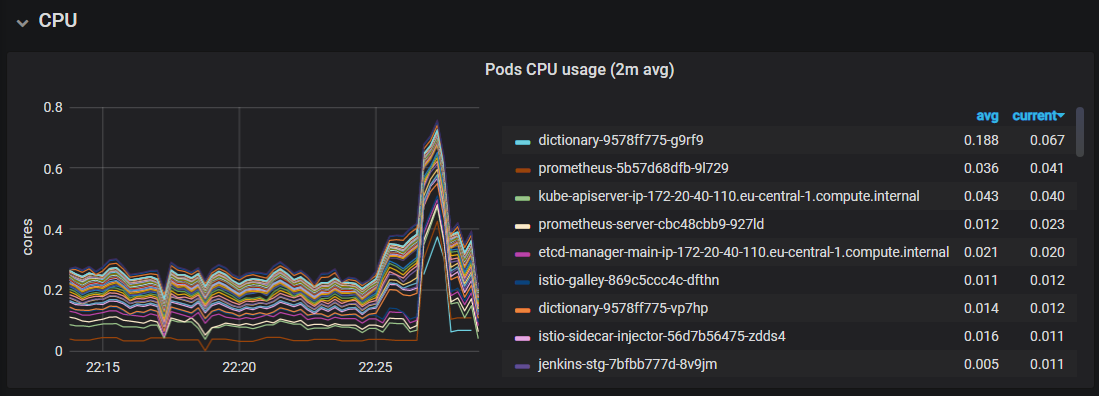
\includegraphics[width=1\textwidth]{img/autoscaling/hpa-grafana-scale-up}
	\end{center}
    \caption{Zużycie CPU podczas testu obciążeniowego \emph{dictionary-service}}
\end{figure}

\section{Horizontal Node Autoscaling}

\begin{figure}[!ht]
	\begin{center}
		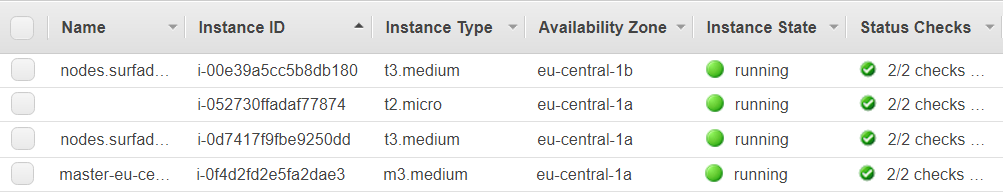
\includegraphics[width=1\textwidth]{img/autoscaling/ca-normal}
	\end{center}
    \caption{Spoczynkowy stan Node'ów}
\end{figure}

\begin{figure}[!ht]
	\begin{center}
		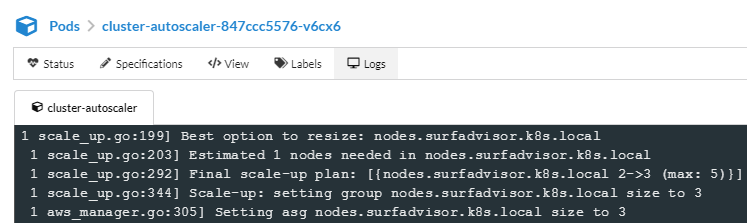
\includegraphics[width=0.9\textwidth]{img/autoscaling/ca-scale-up-logs}
	\end{center}
    \caption{Logi serwisu odpowiedzialnego za skalowanie horyzontalne Node'ów}
\end{figure}

\begin{figure}[!ht]
	\begin{center}
		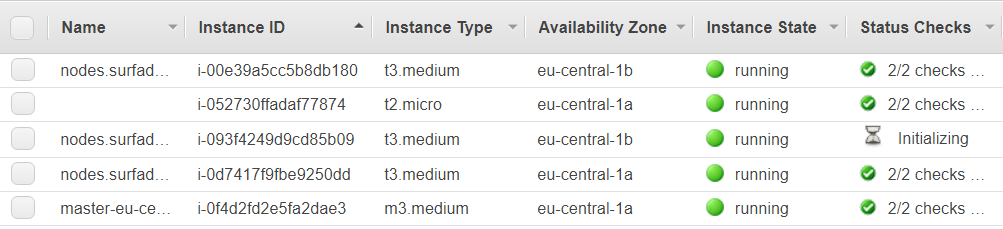
\includegraphics[width=1\textwidth]{img/autoscaling/ca-scale-up}
	\end{center}
    \caption{Stan Node'ów przy skalowaniu w górę}
\end{figure}
